%        File: HarmonyTheory.tex
%     Created: Sat Sep 08 08:00 PM 2012 C
% Last Change: Sat Sep 08 08:00 PM 2012 C
%
\documentclass[a4paper]{book}
\usepackage{amssymb,amsmath,amsthm,enumerate,graphicx,float,lmodern}

\title{A small mathematical model describing tones and their musical relationship}
\author{Ch. B. ten Brinke}

\newtheorem{theorem}{Theorem}[chapter]
\newtheorem{lemma}[theorem]{Lemma}
\newtheorem{proposition}[theorem]{Proposition}
\newtheorem{corollary}[theorem]{Corollary}

\theoremstyle{definition}
\newtheorem{definition}[theorem]{Definition}
\newtheorem{axiom}[theorem]{Axiom}
\newtheorem{example}[theorem]{Example}
\newtheorem{remark}[theorem]{Remark}

\begin{document}
\maketitle

\vspace*{\fill}
\thispagestyle{empty} % optional -- suppress showing of page number
\begin{quotation}
    \em % optional -- to switch to emphasis (italics) mode
    \Large{Music is the arithmetic of sounds as optics is the geometry of light.}

    \medskip
    \raggedleft
    CLAUDE DEBUSSY, c. 1900
\end{quotation}
\vspace*{\fill}

\tableofcontents


\chapter*{Preface}
% Introduceer het onderwerp van de scriptie
In this case study we will try to describe a small part of music in terms of mathematics, namely tones and the relationship that tones have with each other.

Since early history, the connection between music and mathematics has been investigated.
As far as is known, the first scientist that investigated this connection is Pythagoras, who studied interval relations in terms of ratios of whole numbers.
Today, the field of scientific research to music is very broad.
Much research has been done, from many different perspectives.

% Probeer het onderzoeksveld te schetsen
In an article discussing methodological issues in the interdisciplinary research field of mathematical and computational approaches to music, Anja Volk and Aline Honingh give a clear overview of the different research fields that can be distinguished nowadays.
\cite{VolkHoningh}
We resume some of it briefly to give an idea of what has been done on this subject.
First of all, we distinguish the study of consonance and dissonance, which is perhaps one of the oldest branches.
Furthermore, we have musical set theory, which applies mathematical set theory, and more specifically group theory, in order to describe several musical objects.
The concepts of set theory are very general and can be applied to tonal and atonal styles in any equally-tempered tuning system.
Closely related to this are scale theory, transformational theory and Neo-Riemannian theory.
Also topos theory has been applied to music, which, among other things, resulted in topologies for rhythm, melody and harmony.
Generally speaking, the study of music in a scientific way results in methods to analyse music.
However, composition has also been studied in a mathematical way, for instance by Kircher, Xenakis and Mazzola.

%A keenly debated subject within music theory is the study of consonance and dissonance, which combines mathematics and music, but has also been studied from psycho-acoustic perspectives.
%Musical set theory became well-known in the twentieth century, and applies to tonal and atonal music.
%Scale theory, a subdivision of musical set theory, highlights properties of the diatonic collection, such as maximal evenness, and well-formedness .
%Transformational theory, developed in the 1980s, models musical transformations as elements of a mathematical group and applies to both tonal and atonal music as well.
%A branch of transformational theory called Neo-Riemannian theory became popular in the 1990s.
%Applying topos theory resulted in topologies for rhythm, melody, and harmony, and has been used to deal with musical performances.
%Mathematical music analysis covers various methods to analyse music using different mathematical theories.
%Mathematical approaches to composition have also been made, for example by Kircher, Xenakis and Mazzola.

% Leg voordelen van formele theorie uit
One could wonder, what is the use of trying to connect mathematics and music?
Formalization of musical phenomena can make thorough analysis possible.
It could create a better, more intuitive way to think about music.
Moreover, having described music in terms of math, the step to utilize it in computer science is very small.
For instance, it is easier to write computer programs that compose or analyze music, since music can then be reduced to mathematical objects.
However, as Marsden argues in his position paper, a mathematician should never think that the theory fully explains the musical phenomenon, since `there is no single unequivocal set of entities which makes up a piece of music'.
\cite{Marsden}
%Precisely formalized models in mathematics and computation allow empirical work in music research on a large scale through the application of these models to large corpora of digitized music in computational experiments.
%This enables data-rich approaches to music.
%However, the evaluation of these models that are built on abstractions regarding their contribution to our understanding of music is yet a challenging issue.

% Relativeer deze scriptie
From the preceding it is clear that much research has been done in the field of music and mathematics, throughout many years.
In this case study, we will not dive into the current research, but only try to set up an example of a simple mathematical model describing some aspects of music.
Since this is obviously quite a simplification, we would not compromise any thorough studies that have been done in this scientific area.

% Leg het onderwerp en de aanpak van deze scriptie uit
As pointed out before, we will try to model one of the most basic concepts in music, namely tones and tone relations.
If we can give a mathematical definition of tones, we will be able to look at some mathematical properties of tones that come with this definition.
Then it would be interesting to compute these properties for a musical piece, to see what meaning they possibly can have in music, although it may already be obvious for some properties how they should be interpreted, since they are clearly inspired by musical phenomena.
The main focus is on the maths, since this is a thesis in mathematics.
Therefore the testing part will be brief.
Summarizing, the question we are trying to answer in this thesis could be formulated as follows:
can we create a simple mathematical model which describes tones and tone relations?

% Noem de opbouw van de scriptie
We will use the following approach.
In chapter~\ref{tonal_space} we will discuss a formal notion of tones and how these tones relate to each other.
After that, in chapter~\ref{distance} we will consider some elegant mathematical properties of tones, in the form of a notion of distance.
Finally, in chapter~\ref{application} we will briefly apply the model we created in chapters~\ref{tonal_space} and~\ref{distance} to a musical piece in order to get a small indication wether there is some meaning in this model.



\chapter{The Tonal Space}
\label{tonal_space}
% Goal: amusing, introducing and arguing why numbers are a correct, unique representation of music.
In this chapter we will discuss the very first principles of tones.
From this we will then deduce a formal definition.
This will allow us to talk about tones in a mathematical way and enable us to investigate some mathematical properties of it, as we will do in chapter~\ref{distance}.

\section{Tones as numbers}
% Introduction of physics in music
Music consists of sound.
Sound consists of longitudinal waves in air, caused by difference in pressure.
For such a wave to be perceived as a musical tone, it has to be periodic.
The length of this period, i.e.\ the frequency of the wave, defines the pitch of the tone.
For instance, the note ``A'', has a basic frequency of 440 Hz.
The higher the frequency of the tone, the ``higher'' the tone will sound.
Of course, a tone is more than only its frequency.
The shape of the wave defines the timbre of the sound.
The loudness of a tone corresponds with the amplitude of the wave.
But when we are studying music theory in general, we don't want to distinguish between tones played by a violin and tones played by an oboe and we also want to disregard the loudness of tones.
Therefore, it seems correct to reduce the notion of a tone to its basic frequency for our purpose.

%When we have two tones, we can make them sound together, by adding their waves.
%We want that this sum is again periodic, but this is not always true.
%For instance, if we have two waves corresponding to the functions $\sin(x)$ and $\sin(\pi x)$, the sum $\sin(x) + \sin(\pi x)$ is not periodic.
%In general, the sum of two waves with periods $a$ and $b$ is periodic if and only if $\frac{a}{b} \in \mathbb{Q}$.
%So if we require that the frequencies of a tone are always rational, their sum will be periodic and thus will have a frequency again.

So essentially we assume a tone corresponds to a positive number.
This enables us to talk about relationships between musical tones as being numerical relationships.

\section{Harmonious relationships}
%Anekdote about pythagoras
Legends have come down to us, through the late Roman writer Boethius among others, relating how Pythagoras ``discovered'' a remarkable fact.
They alleged that Pythagoras noted the harmonious relationships of the sounds produced by the hammers in a blacksmith's forge, and further investigations revealed that the masses of these hammers were, extraorinarily, in simple wholenumber ratios to each other!
From this claimed observation Pythagoras is supposed to have leapt the realization that consonant sounds and simple number ratios are correlated - that ultimatily music and mathematics share the same fundamental basis. \cite{NeilBibby}

%Explain why multiplication is a natural operation on tones
Let us assume we have some initial tone, which we from now on refer to as \emph{tonic}.
Following the observation of Pythagoras, we can construct new tones from the tonic by multiplying its frequency by ``simple'' rational numbers.
According to Pythagoras, these are harmoniously closely related to the tonic, since the ratio between each of them and the tonic is a ``simple'' rational number.

Let us consider some examples of harmonious relationships between two tones, also known as \emph{intervals}, that have been recognized throughout history.
They have been given names in traditional music theory that the reader may be familiar with.
If we muliply the tonic's frequency with $2$, we get a tone that sounds an ``octave'' higher than the tonic.
If we muliply the tonic's frequency with $\frac{3}{2}$, we get a tone that sounds a ``fifth'' higher than the tonic.
Any simple harmonious relationship that we know from experience, seems to correspond to some simple rational number.
The most prominent ones have been listed in table~\ref{musical_intervals}.

\begin{table}[h]
    \centering
    \begin{tabular}{|c|c|}
        \hline
        name & number \\ \hline
        octave & $2/1$ \\ 
        fifth & $3/2$ \\ 
        fourth & $4/3$ \\ 
        major third & $5/4$ \\ 
        minor third & $6/5$ \\ 
        second & $9/8$ \\ 
        \hline
    \end{tabular}
    \caption{Some musical intervals}
    \label{musical_intervals}
\end{table}

In this thesis, we like to disregard the actual frequency of a tone.
We only want to study the ratio tones have with the tonic.
This way we don't distinguish between pieces of music with different tonics.
In other words, we assume that a translated version of a piece of music is equivalent to the original piece.
Now if we only want to regard the ratio that tones have with some tonic, we better disregard the frequency of tones completely and regard a tone as being the number the tonic must be multiplied with to obtain it.
This leaves out the information that we don't care about.
In other words, if we have a tonic and multiples of the tonic's frequency, we could very well divide every tone's frequency by the tonic's frequency (including the tonic itself) without changing the mutual ratio's.
This would map the tonic to $1$ and all the other tones to the ratio they have with the tonic.
%From here, a tone IS the number
Thus given the tonic, the ratio of a tone with the tonic uniquely identifies the tone, and is therefore a correct representation.
Therefore we will not consider a tone being its physical frequency, but rather the ratio that its frequency has with the frequency of the tonic.
So from now on, a tone refers to a positive rational number.

As pointed out before, we can multiply a tone with a positive rational number to get another tone.
In musical terms, multiplying a tone with a number is the same as stacking an interval upon a tone, to reach another tone.
Since we reduced a tone to be a positive rational number, it follows that multiplying a tone with a positive rational number co\"incides with multiplying a tone with another tone.
Therefore it makes sense to define number multiplication as an operation on tones.
%So, in musical terms, we regard an interval as being a tone (namely the tone one gets when one adds the interval to the tonic).
%This means that we add tone to another tone in order to reach a third tone.

Having suggested multiplication as an operation on tones, we can think about sets of tones, closed under this operation.
If we choose some ``simple'' tones, we can construct a group under multiplication, generated by these simple tones.
Let us define this more formally.

\newcommand{\gen}[1]{\langle #1 \rangle}

\paragraph{A few notation conventions:}
\begin{enumerate}[i]
	\item 
		Ordinary multiplication between numbers is denoted by $\cdot$.
	\item 
		When $(G, \cdot)$ is a group, we denote the group by $G$ as well.
    \item
        We will always assume $\cdot$ as operator, unless explicitly defined otherwise.
    \item
        The group generated by a set $S$ is denoted by $\gen{S}$.
\end{enumerate}

\newcommand{\Q}{\mathbb{T}}%{\mathbb{Q}_{> 0}}
\newcommand{\R}{\mathbb{R}_{> 0}}
\newcommand{\T}{\mathbb{T}}

\begin{definition}
    Denote the group $(\mathbb{Q}_{> 0}, \cdot)$ by $\Q$.
	A \emph{tonal space} $T$ is a subgroup of $\Q$.
    An element $t \in T$ is called a \emph{tone}.
    A set of tones is called a \emph{scale}.
\end{definition}

Since it is not immediately clear what it means for a tone to be ``simple'', we do not put any restrictions on the definition of a tonal space regarding ``simpleness'' of its generators.
Later on we will come back to simpleness.
Notice that using ordinary number multiplication as operation, makes a tonal space an abelian group.

\begin{example}
    \label{ptolemaic_sequence}
    Let $T = \gen{2,3,5}$.
    Then $T$ is a tonal space.
    The set \[\{1,\frac{9}{8},\frac{5}{4},\frac{4}{3},\frac{3}{2},\frac{5}{3},\frac{15}{8},2\}\] is a scale of $T$.
    This set is known as \emph{Ptolemaic scale}.
\end{example}

\begin{example}
    Let $T = \gen{2,3}$.
    Then $T$ is a tonal space.
    The set \[\{1,\frac{9}{8},\frac{81}{64},\frac{4}{3},\frac{3}{2},\frac{27}{16},\frac{243}{128},2\}\] is a scale of $T$.
    This is the oldest known form of tuning, called the \emph{Pythagorean diatonic scale}.
\end{example}

We present a result regarding generators of tones.

\newcommand{\Primes}{\mathbb{P}}
\newcommand{\I}{\mathbb{I}}

\begin{theorem}
    $\Q = \gen{\Primes} = \gen{\I}$, where $\Primes$ is the set of all primes, and $\I$ is the set of all numbers of the form $\frac{p+1}{p}$, $p \in \Primes$.
    \label{thm_generator_equivalence}
\end{theorem}
\begin{proof}
    We proceed by proving $\gen{\I} \subset \Q \subset \gen{\Primes} \subset \gen{\I}$.
    For the first inclusion notice that $\I \subset \Q$ and therefore $\gen{\I} \subset \Q$.

    For the second inclusion, let $a \in \Q$.
    Then there exist $p,q \in \mathbb{N}$ such that $a = \frac{p}{q}$.
    By the \emph{unique-prime-factorization theorem} $p$ and $q$ can be written as a product of primes $p_1,\dots,p_n$ and $q_1,\dots,q_m$ respectively.
    This implies that $p$ and $q$ are in $\gen{\Primes}$.
    Because $q$ is in $\gen{\Primes}$, also $\frac{1}{q}$ is in $\gen{\Primes}$.
    Since a group is closed under its operation, $p\cdot \frac{1}{q} = a$ is in $\gen{\Primes}$.
    Thus $\Q \subset \gen{\Primes}$.

    For the final inclusion, suppose that there exists $p_0 \in \Primes$ such that $p < p_0 \Rightarrow p \in \gen{\I}$.
    Notice that this implies that $p_0-1 \in \gen{\I}$, even though $p_0 -1$ is not prime.
    Namely, if not, $p_0 - 1$ could be written as a product of primes which are all larger than itself, which is a contradiction.
    Since $\frac{p_0}{p_0-1} \in \gen{\I}$ by definition, we get $(p_0 -1) \cdot \frac{p_0}{p_0-1} = p_0 \in \gen{\I}$.
    Since $2 = \frac{2}{1} \in \gen{\I}$ and $2$ is the smallest prime, we can proceed by induction.
\end{proof}

\begin{corollary}
    Any tone can be written uniquely, aside from order, as 
    \begin{enumerate}[i]
        \item a product of primes.
        \item a product of numbers of the form $\frac{p+1}{p}$, where $p$ is a prime.
    \end{enumerate}
\end{corollary}
\begin{proof}
    Applying~\ref{thm_generator_equivalence} immediately gives the result, since both the set of primes and the set of numbers of the form $\frac{p+1}{p}$, with $p$ prime, generate the maximal tonal space $\Q$.
\end{proof}

\section{Equally temperedness}
\label{section_equally_temperedness}
The reader who is already a bit familiar with music theory, may know that nowadays the most widely used scale is the \emph{twelve tone equally tempered scale}.
An equally tempered scale does not consist of tones that have a ``simple'' ratio between each other.
Instead, it consists of tones that are subsequent powers of some base number.
In the case of the twelve tone equally tempered scale, this base number is $2^\frac{1}{12}$.
Notice that this base number results in a scale with exactly 12 tones in one octave, namely \[\{2^\frac{1}{12},2^\frac{2}{12},2^\frac{3}{12},2^\frac{4}{12},2^\frac{5}{12},2^\frac{6}{12},2^\frac{7}{12},2^\frac{8}{12},2^\frac{9}{12},2^\frac{10}{12},2^\frac{11}{12}, 2^\frac{12}{12} = 2\}.\]
Hence the name twelve tone equally tempered scale.

According to what we said previously, these tones should sound horribly together, but we know they don't.
We can explain this with the fact that our ears have a certain tolerance regarding tuning of tones.
So, tones that are just a little bit mistuned will not sound so bad.
Our ears will still recognize the tone that was intended.

Figure~\ref{equally_temperedness} confirms that the tones ocurring in the Ptolemaic scale are well approximated by tones in the twelve tone equally tempered scale.

\begin{figure}[H]
    \centering
    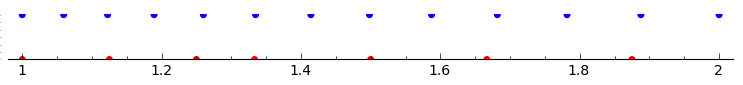
\includegraphics[scale=0.65]{figures/equally_temperedness.png}
    \caption{Blue upper points represent tones from the twelve tone equally tempered scale and red lower points represent tones from the Ptolemaic scale.}
    \label{equally_temperedness}
\end{figure}

Let us state a formal definition of equally temperedness.

\begin{definition}
    An \emph{equally tempered tonal space} is a cyclic subgroup of $(\R,\cdot)$.
    An element of an equally tempered tonal space is called an \emph{equally tempered tone}.
    A subset of an equally tempered tonal space is called an \emph{equally tempered scale}.
\end{definition}

Thus we can consider an equally tempered tonal space as being an approximation of a tonal space.
Notice that according to the definitions used in this thesis, an equally tempered tonal space is \emph{not} a tonal space, and does not contain tones, but contains rather approximations of tones.
Most of the musical compositions are played using tones from such approximations, instead of from an actual tonal space.
This has several practical and historical reasons.
We will not study equally temperedness further, as it is beyond the scope of this thesis.
However, this knowledge is needed for understanding the connection between tonal spaces and music that is played in equally tempered scale.
Namely, it is not directly clear what tones in a tonal space correspond to what tones in an equally tempered tonal space.
Therefore we cannot directly apply the model we presented thus far, since the model assumes a tonal space, and not an approximation.
When we want to test the model in chapter~\ref{application} we will first have to recover a tonal space from the approximation.




\chapter{Distance between Tones}
\label{distance}
In this chapter we will consider an elegant mathematical structure on tones, namely the notion of distance.
Now that we defined the notion of tones, we can look at some properties of tonal spaces, in the form of mathematical metrics.
To do this, we will first discuss the properties itself, and then show how these fit in the notion of distance.
This will then result in a mathematical definition of the concerning property.
We will treat these things as mathematical properties first, while afterwards, in chapter~\ref{application}, we can try to test if there is some musical meaning in them and maybe try to interpret them.
However, as pointed out before, it may already be obvious for some properties to which musical phenomena they correspond, since they are clearly inspired by these phenomena.

\section{Metric on abelian groups}

First of all, let us recall the notions norm and metric for abelian groups and thus for tonal spaces.

\begin{definition}
    Let $G$ be an abelian group.
    Then a function $\|\cdot\|:G \to [0,\infty)$ is called a \emph{norm} on $G$, if it suffices the following properties for all $g,h \in G$.
	\begin{enumerate}[i]
		\item $\|g\| = 0 \Leftrightarrow g=1$
        \item $\|g\| = \|g^{-1}\|$
		\item $\|g \cdot h\| \leq \|g\| + \|h\|$
	\end{enumerate}
\end{definition}

\begin{definition}
	A \emph{metric} on an abelian group $G$ is a function $d:G \times G \to [0,\infty)$, sufficing the following properties for all $g,h,j \in G$:
	\begin{enumerate}[i]
		\item $d(g,h) = 0 \Leftrightarrow g=h$
		\item $d(g,h) = d(h,g)$
		\item $d(g,j) \leq d(g,h) + d(h,j)$
	\end{enumerate}
\end{definition}

A norm defined on an abelian group can induce a metric, as pointed out by the following lemma.

\begin{lemma}
    Let $G$ be an abelian group with a norm.
    Define $d:G \times G \to [0,\infty), (g,h) \mapsto \|gh^{-1}\|$.
    Then $d$ is a metric.
	\label{norm_to_metric}
\end{lemma}
\begin{proof}
	We show that $d$ suffices the properties of a metric.
    \begin{enumerate}[i]
        \item $d(g,h) = 0 \Leftrightarrow \|gh^{-1}\| = 0 \Leftrightarrow gh^{-1} = 1 \Leftrightarrow g = h$.
        \item $d(g,h) = \|gh^{-1}\| = \|(hg^{-1})^{-1}\| = \|hg^{-1}\| = d(h,g)$.
        \item $d(g,j) = \|gj^{-1}\| = \|gh^{-1}hj^{-1}\| \leq \|gh^{-1}\|+ \|hj^{-1}\| = d(g,h) + d(h,j)$.
    \end{enumerate}
	Thus $d$ is a metric on $G$.
\end{proof}

\section{Pitch distance}
The following mathematical property that we discuss is inspired by the phenomenon of pitch.
Therefore this mathematical property has already a pretty obvious musical interpretation on beforehand.

Pitch is a perceptual property that allows the ordering of sounds on a frequency-related scale.
We all know pitches intuitively and compare them as ``higher'' and ``lower''.
The greater the frequency of the tone, the ``higher'' its sound.
So, some tones sound ``higher'' in pitch than others.
This difference in pitch can be thought of as distance.
We will call this kind of distance \emph{pitch distance}.

If we want to measure this difference in pitch as a (mathematical) metric, we must decide how we want the metric to behave.
Remember that, in musical terms, if we ``stack'' a musical interval upon a tone, this corresponds to multiplying with a number.
For instance if we ``add'' an ``octave'' to a tone, this corresponds to multiplying the tone with $2$.
So in this case the ``difference'' in pitch is a (multiplicative) factor 2, while we like to think of it as an (additive) octave.
This suggests that we might want to turn multiplication into addition, when converting ratio between tones to distance in pitch, because the idea of increasing the pitch of a tone by ``adding'' an octave to it is very intuitive.

To turn multiplication into addition, we need an injective group homomorphism between $\T$ and $(\mathbb{R},+)$.
This then can induce a norm, as pointed out by the following lemma.

\begin{lemma}
    Let $G$ be an abelian group, and $\varphi : G \to (\mathbb{R},+)$ an injective group homomorphism.
    Then $\| \cdot \| : G \to \mathbb{R}_{\geq 0}, g \mapsto |\varphi(g)|$ a norm, where $| \cdot |$ is the norm that takes numbers to their absolute value.
    \label{homomorphism_to_metric}
\end{lemma}
\begin{proof}
    We show that the properties of a norm are fulfilled.
    \begin{enumerate}[i]
        \item $\|g\| = 0 \Leftrightarrow \varphi(g) = 0 \Leftrightarrow g = 1$
        \item $\|g^{-1}\| = |\varphi(g^{-1})| = |-\varphi(g)| = |\varphi(g)| = \|g\|$
        \item $\|gh\| = |\varphi(gh)| = |\varphi(g) + \varphi(h)| \leq |\varphi(g)| + |\varphi(h)| = \|g\| + \|h\|$
    \end{enumerate}
\end{proof}

For a norm to actually measure difference in pitch, an additional property is needed.
Namely, we need to be sure that if a tone $t$ is further away from the tonic than a tone $s$, then $\|s\| \leq \|t\|$.
The following definition of pitch distance will suffice this property, as shown in theorem~\ref{order_preserving_homomorphism}.

\begin{definition}
    Let $T$ be a tonal space and $\varphi : T \to (\mathbb{R},+)$ an injective group homomorphism,
    with the property that $s \leq t \Leftrightarrow \varphi(s) \leq \varphi(t)$, for all $s,t \in T$.
    Then the norm that follows by applying lemma~\ref{homomorphism_to_metric}, is called a \emph{pitch norm}.
    The metric that can be induced from this norm by lemma~\ref{norm_to_metric}, is called a \emph{pitch distance}.
\end{definition}

\begin{theorem}
    \label{order_preserving_homomorphism}
    Let $T$ be a tonal space and $\varphi : T \to (\mathbb{R},+)$ inducing a pitch norm $\| \cdot \|$ on $T$.
    Then $ \max(s,s^{-1}) < \max(t,t^{-1}) \Leftrightarrow \|s\|<\|t\|$.
    In other words, a tone $t$ is strictly further away from the tonic than a tone $s$, if and only if $\|s\| < \|t\|$.
\end{theorem}
\begin{proof}
    Denote $s' = \max(s,s^{-1})$ and $t' = \max(t,t^{-1})$.
    Notice that $1 \leq s'$ and $1 \leq t'$.
    Suppose $s' < t'$.
    We know that $s \leq t \Leftrightarrow \varphi(s) \leq \varphi(t)$, for all $s,t \in T$.
    So 
    \begin{alignat*}{3}
        & 1 & &\leq s'             & &<  t' \\
        & 0 & &\leq \varphi(s')    & &<  \varphi(t') \\
        & 0 & &\leq |\varphi(s')|  & &<  |\varphi(t')| \\
        & 0 & &\leq \|s\|          & &<  \|t\|
    \end{alignat*}
    
    Now suppose $\|s\|<\|t\|$.
    Then 
    \begin{alignat*}{3}
        & 0 & &\leq \|s\|          & &<  \|t\| \\
        & 0 & &\leq |\varphi(s')|  & &<  |\varphi(t')| \\
        & 0 & &\leq \varphi(s')    & &<  \varphi(t') \\
        & 1 & &\leq s'             & &<  t' 
    \end{alignat*}
\end{proof}

\begin{example}
    \label{log_as_melodic_distance}
    Let $T$ be a tonal space and $s,t \in T$.
    Any logarithm is an injective group homomorphism from $T$ to $(\mathbb{R},+)$, since $\log(st) = \log(s) + \log(t)$, no matter what the base of the logarithm is.
    Notice that $s \leq t \Leftrightarrow \log(s) \leq \log(t)$, so $t \mapsto |\log(t)|$ is a pitch norm and $(s,t) \mapsto |\log(s)-\log(t)|$ a pitch distance.
\end{example}

\section{Harmonic distance}
In this section we will consider a second kind of distance between tones.
Unlike pitch distance, this property doest not have a clear musical interpretation on beforehand.
It is inspired by the physical phenomenon of harmonics.

In physics, a tone with a frequency that is an integer multiple of a main frequency is called a harmonic.
In terms of the definitions used in this thesis, the $n$th multiple of some base tone is called the $n$th harmonic.
The other way around, a tone such that the main frequency is an integer multiple of the frequency of the tone is called a subharmonic.
We can try to express the harmonical and subharmonical relation between tones as distance.
We will refer this kind of metric as \emph{harmonic distance}.

Remember that we defined tones to be rational numbers.
This implied that we can speak of a ratio between two tones, which is again a tone.
Notice that the ratio between two tones is the tone the first tone has to be multiplied with to obtain the second tone.
Namely, if we multiply a tone $t$ with the tone $\frac{s}{t}$, we get $t \cdot \frac{s}{t} = s$.
Suppose $\frac{s}{t} = \frac{a}{b}, a,b \in \mathbb{N}$.
Then, in terms of harmonics and subharmonics, the tone $s$ can be reached from the tone $t$ by taking the $b$th subharmonic and then the $a$th harmonic.

For determining the harmonic distance between two tones, we want to judge their ratio on ``simpleness'' in terms of harmonics and subharmonics.
%We can deduce from this that we can construct tones that are very close to the tonic by multiplying the tonic with simple numbers.
Since a ratio is again a tone, this raises the question, which tones are simple?
%Or more specifically, how can we determine the simpleness from numbers?
If we first find a formula for the simpleness of tones, we can use it as a norm.
This norm will then induce a metric by lemma~\ref{norm_to_metric}.
So essentially we are looking for an harmonic norm $\| \cdot \| : \Q \to \mathbb{R}_{\geq 0}$, which reflects simpleness of tones.
The greater its norm, the greater the complexity of the tone.
We will state some assumptions we make about the harmonic norm and then formulate a formal definition.

First, we have to make an assumption about products of tones.
We want that if we multiply a tone $t \in \mathbb{N}$ with another tone $s \in \mathbb{N}$, that $\|st\| = \|s\|+\|t\|$.
This makes sense, since both $t$ and $s$ have some degree of complexity, and therefore their product has both degrees of complexity in it, suggesting that the resulting complexity should be the sum of the parts.
However if for instance $t$ and $s$ are not natural, some problem may occur.
For example, $t$ may be the inverse of $s$.
In that case, we definitely don't want that $\|st\| = \|s\|+\|t\|$, since $\|st\|=\|t^{-1}t\|=\|1\|$, which is very, very simple.
Generally speaking, if $t = a \cdot b$ is a tone with $a$ and $b$ such that the numerator of $a$ is coprime with the denominator of $b$ and vice versa, we want that the value of $t$ is the same as the values of $a$ and $b$ added together.
Remember that two numbers being coprime means that the greatest common divisor between those two numbers is $1$.

The second assumption we make, is that any tone $t$ is just as simple as its inverse $t^{-1}$.
This also makes sense, since we decided that we would not care about actual frequency number values of tones, but only about their ratio to the tonic. 
That implied that we assume that tones behave the same under translation.
So, considering the harmonic distance between $1$ and $t$, we could translate both $1$ and $t$ down by $t$, resulting in $t^{-1}$ and $1$.
Now if tones behave the same under translation, clearly the harmonic distance between $1$ and $t$ and between $t^{-1}$ and $1$ should be the same, implying that $\|t\| = \|t^{-1}\|$.

The third and last assumption we have to make, is that $1$ is the only tone with norm $0$.
This makes sense because the harmonic distance between two tones should indeed be zero if and only if they are the same.

Let us list the assumption we just stated as axioms for the harmonic norm.
\begin{definition}
    A \emph{harmonic norm} $\| \cdot \|$ is a norm on $\Q$ sufficing the following properties.
    \begin{enumerate}[i]
        \item If $t = a \cdot b$ is a tone with $a$ and $b$ such that the numerator of $a$ is coprime with the denominator of $b$ and vice versa, then $\|t\| = \|a\|+\|b\|$.
        \item For any tone $t$, $\|t\| = \|t^{-1}\|$.
        \item For any tone $t$, $\|t\| = 0 \Leftrightarrow t = 1$.
    \end{enumerate}
    The metric that can be induced from this norm by lemma~\ref{norm_to_metric}, is called a \emph{harmonic distance}.
\end{definition}

Let us verify that the notion of harmonic norm we just defined satisfies the axioms of a norm.

\begin{lemma}
    A harmonic norm $\| \cdot \|$ is indeed a norm.
\end{lemma}
\begin{proof}
    We show that $\| \cdot \|$ suffices the properties of a norm.
    \begin{enumerate}[i]
        \item $\|t\| = 0 \Leftrightarrow t = 1$ (by definition)
        \item $\|t^{-1}\| = \|t\|$ (by definition)
        \item Let $t = \frac{ax}{by},s = \frac{cy}{dx}$ two tones such that $ax$ is coprime with $by$, $cy$ is coprime with $dx$, $a$ is coprime with $d$ and $b$ is coprime with $c$.
            Note that any two tones can be written this way. 
            Now 
    \begin{eqnarray*}
            \|ts\| &=& \|\frac{ax}{by} \frac{cy}{dx}\|  \\
            &=& \|\frac{a}{b} \frac{c}{d}\| \\
            &=& \|\frac{a}{b}\| + \|\frac{c}{d}\|  \\
            &\leq& \|\frac{a}{b}\| + \|\frac{x}{y}\| + \|\frac{c}{d}\| + \|\frac{y}{x}\|  \\
            &=& \|\frac{a}{b}\frac{x}{y}\| + \|\frac{c}{d}\frac{y}{x}\|  \\
            &=& \|t\| + \|s\|.
    \end{eqnarray*}
    \end{enumerate}
\end{proof}

It appears that we only need to assign a value for the harmonic norm to each generator of a tonal space.
Then the harmonic norm of every other tone can be determined from this, as pointed out by theorem~\ref{function_to_harmonic_norm}.
Thus a function assigning strictly positive numbers to generators of a tonal space, induces a harmonic metric.

\begin{theorem}
    Let $T$ be a tonal space and $\| \cdot \|$ a harmonic norm on $T$.
    Then $\|t\| = \varphi(p_0) + \dots + \varphi(p_n) + \varphi(q_0) + \dots + \varphi(q_m)$, where $\varphi$ is a function that assigns a strictly positive number to every prime generator of $T$.
    \label{function_to_harmonic_norm}
\end{theorem}
\begin{proof}
    Let $T$ be a tonal space and $\| \cdot \|$ a harmonic norm on $T$.
    Let $\varphi$ such that $\varphi(p) = \|p\|$ for all prime generators of $T$.
    Now let $t \in T$ with unique prime factorization $\frac{p_0 \dots p_n}{q_0 \dots q_m}$.
    Then 
    \begin{eqnarray*}
        \|t\| &=& \|\frac{p_0 \dots p_n}{q_0 \dots q_m}\| \\
            &=& \|p_0 \dots p_nq_0^{-1} \dots q_m^{-1}\| \\
            &=& \|p_0\|+ \dots + \|p_n\| + \|q_0^{-1}\| + \dots + \|q_m^{-1}\| \\
            &=& \|p_0\|+ \dots + \|p_n\| + \|q_0^{-1}\| + \dots + \|q_m^{-1}\| \\
            &=& \|p_0\|+ \dots + \|p_n\| + \|q_0\| + \dots + \|q_m\|\\
            &=& \varphi(p_0) + \dots + \varphi(p_n) + \varphi(q_0) + \dots + \varphi(q_m)
    \end{eqnarray*}
\end{proof}


\begin{example}
    \label{eulers_formula}
    Let $T = \gen{2,3,5}$ be a tonal space.
    Define a harmonic norm such that $\|2\| = 1$, $\|3\| = 2$ and $\|5\| = 4$.
    By theorem~\ref{function_to_harmonic_norm}, this indeed induces a harmonic norm.
    Again by by lemma~\ref{norm_to_metric} this induces a harmonic distance.
\end{example}

In his work \emph{Tentamen novae theoriae musicae ex certissismis harmoniae principiis dilucide expositae} Leonhard Euler studied music theory by investigating ratio's between tone frequencies.
He came up with a formula attempting to measure the amount of what he called ``agreeableness'' which can be found in a set of tones played together. \cite{Euler}
This comes close to what we would call the amount of ``simpleness''.
The formula he used is as follows.
\[ \mathrm{agreeableness(}t\mathrm{)} = 1 + \sum_{i = 0}^{n}{(p_i-1)},\text{\ where\ } t = \frac{p_0 \dots p_m}{p_{m+1} \dots p_n} \]
So for every prime $p$, he assigned the value $p-1$ as agreeableness, just like we did in example~\ref{eulers_formula}.
His formula is very similar to the harmonic distance in example~\ref{eulers_formula}, but there are a few differences.
First of all, he liked to add $1$ to the formula, implying that that amount of consonance of the tone $1$ (the tonic) is $1$.
This causes his formula not to be compatible with the axioms of distance.
Secondly, he did not consider fractional tones but only natural numbers, since any set of fractional tones can be made natural by scaling them up, without changing their mutual ratio's.
Euler did not formulate any assumptions and gave no proof for his formula.
So with some assumptions that don't seem too bad, we arrived at a formula similar to Euler's formula, but in a more general form and compatible with the axioms of distance.


\section{Pitch-Harmonic distance}
There are many more notions of distance possible on a tonal space.
For instance, we can combine pitch metric and harmonic metric into another metric.
We will use it in Chapter~\ref{application} to compare the pitch distance with the harmonic distance.
This one is not particularly inspired by a well known phenomenon in music, but rather just a mathematical property.

\begin{theorem}
    The sum of two norms, is again a norm.
    \label{sum_of_norms}
\end{theorem}
\begin{proof}
    Let $\|\cdot\|_1$ and $\|\cdot\|_2$ be two norms on an abelian group $G$.
    Define $\|\cdot\| = \|\cdot\|_1 + \|\cdot\|_2$.
    We prove the properties of a norm.
    \begin{enumerate}[i]
        \item $\|g\| = \|g\|_1 + \|g\|_2 = 0 \Leftrightarrow \|g\|_1 = 0 $ and $\|g\|_2 = 0 \Leftrightarrow g = 1$
        \item $\|g^{-1}\| = \|g^{-1}\|_1 + \|g^{-1}\|_2 = \|g\|_1 + \|g\|_2 = \|g\|$
        \item $\|gh\| = \|gh\|_1 + \|gh\|_2 \leq  \|g\|_1 + \|g\|_2 + \|h\|_1 + \|h\|_2 = \|g\| + \|h\|$
    \end{enumerate}
\end{proof}

\begin{corollary}
    The sum of a pitch metric and a harmonic metric is again a metric
    \label{sum_of_metrics}
\end{corollary}
\begin{proof}
    Write the pitch metric and the harmonic metric as norms and apply theorem~\ref{sum_of_norms}.
    Then applying lemma~\ref{norm_to_metric} yields the result.
\end{proof}

\begin{example}
    Let $T = \gen{2,3,5}$ be a tonal space.
    Define a harmonic norm such that $\|2\|_H = 1$, $\|3\|_H = 2$ and $\|5\|_H = 4$.
    Define the pitch norm such that $\|t\|_M = \log(t)$, for every $t\in T$.
    Then \[\|t\|_M + \|t\|_H = \log(t) +\sum_{i = 0}^{n}{(p_i-1)},\text{\ where\ } t = \frac{p_0 \dots p_m}{p_{m+1} \dots p_n} \] is a norm.
\end{example}

\chapter{Applying the Model}
\label{application}
We will look at an application of the preceding model to a few measures of a musical composition.
The musical piece we choose is Pachelbel's Canon, the canon written by the German Baroque composer, Johann Pachelbel, taken from his \emph{Canon and Gigue for 3 violins and basso continuo}.
This is a famous piece and suitable for studying basic music theory, since the simple theme that is used in it is very common in western music.

\section{Recovering approximation}
The first problem we encounter is that the piece is normally played in equally tempered scale.
Remember from section~\ref{section_equally_temperedness} that this means that we do not know the actual tones used in the piece, but rather approximations of these tones.
We will first have to convert these approximations to tones before we can study them like we did in the previous chapters.
For now we will not study approximation recovery algorithms, but use an easy method to derive the actual tones that are used in the composition.
But please keep in mind that may not be the best way to do it.
For each equally tempered tone, we will just take the closest tone occuring in the Ptolemaic Sequence, presented in example~\ref{ptolemaic_sequence}.
Since this piece is in major scale and contains no ``accidentals'', this may be suitable enough.
We will choose the note ``d'' as the tonic, since this piece is written in ``D major''.

\section{Analysis of a monophonic part}
Let us study the first six measures played by the first violin. The partiture of this piece in traditional notation, along with the resulting tones are displayed in figure~\ref{fig_first_violin_tones}.

\begin{figure}[H]
    \centering
    
\includegraphics[scale=0.25]{figures/fig_first_violin_tones.png}
    \caption{First six measures of first violin, showing corresponding tones}
    \label{fig_first_violin_tones}
\end{figure}

Let us now apply the mathematical metrics we developed in chapter~\ref{distance}.
We first want to compute the pitch distance between every tone and its subsequent tone.
We are free to choose the formula $\log_{2^{\frac{1}{12}}}(t)$ as pitch distance, by example~\ref{log_as_melodic_distance}.
To make the numbers nice, we round the pitch distances.
The results are displayed in figure~\ref{fig_first_violin_melodic_distance}.
One should interpret the number below a tone as the pitch distance that had to be travelled from the previous tone, to arrive at the current tone.

\begin{figure}[H]
    \centering
    
\includegraphics[scale=0.25]{figures/fig_first_violin_melodic_distance.png}
    \caption{First six measures of first violin, showing rounded pitch distance to the previous tone}
    \label{fig_first_violin_melodic_distance}
\end{figure}

As we can see, the pitch distance indeed points out out how the melody jumps up and down.
Unsurprisingly, this rounded pitch distance exactly corresponds with the number of tones in the twelve tone equally tempered scale (informally known as semitones) between the two subsequent tones.
This is because we took $2^\frac{1}{12}$ as base for the logarithm in the pitch distance.

The same way, we can compute the harmonic distance between subsequent tones.
We decide to use the formula from example~\ref{eulers_formula}.
The results are displayed in figure~\ref{fig_first_violin_harmonic_distance}.
The number right below a tone, is the harmonic distance between that tone and the previous tone.
In other words, it represents the harmonic distance that had to be travelled to arrive from the previous tone at the current tone.

\begin{figure}[H]
    \centering
    
\includegraphics[scale=0.25]{figures/fig_first_violin_harmonic_distance.png}
    \caption{First six measures of first violin, showing harmonic distance to the previous tone}
    \label{fig_first_violin_harmonic_distance}
\end{figure}

Analyzing figures~\ref{fig_first_violin_harmonic_distance} and~\ref{fig_first_violin_melodic_distance}, we can make a few interesting observations.

% Noem hier iets over klaarblijkelijke muzikale betekenis van harmonic distance

The most notable harmonic distance is 3, because it is the lowest one by far.
In musical theory this interval is known as fifth and is traditionally recognized as a fairly simple interval.

Secondly, it appears that most of the time, when the harmonic distance is relatively high, the pitch distance is relatively low, and vice versa.
To confirm this, we like to display the pitch-harmonic distance, as a sum of the two previous distances.
By corollary~\ref{sum_of_metrics} this is indeed a metric.
This then results in figure~\ref{fig_first_violin_melodic_harmonic_distance}.
Indeed, the spread appears to be small, suggesting that pitch distance and harmonic distance neutralize each other most of the time.

\begin{figure}[H]
    \centering
    
\includegraphics[scale=0.25]{figures/fig_first_violin_melodic_harmonic_distance.png}
    \caption{First six measures of first violin, pitch pitch-harmonic distance to the previous tone}
    \label{fig_first_violin_melodic_harmonic_distance}
\end{figure}

It may also be interesting to display the harmonic distance between every tone and the tonic.
Remember that in this piece the note which is informally referred to as ``d'' corresponds with $1$, and is therefore called tonic.
See figure~\ref{fig_first_violin_tones}.
We can then compare this with the distance between subsequent tones.
For convenience we place the harmonic distance to the previous tone above, and the harmonic distance to the tonic below.
The results are displayed in figure~\ref{fig_first_violin_harmonic_distance_to_tonic}.

\begin{figure}[H]
    \centering
    
\includegraphics[scale=0.25]{figures/fig_first_violin_harmonic_distance_to_tonic.png}
    \caption{First six measures of first violin, showing harmonic distance to previous tone above and harmonic distance to tonic below.}
    \label{fig_first_violin_harmonic_distance_to_tonic}
\end{figure}

We can observe that the distance to the previous tone is most of the time greater than the distance to the tonic.
There are three exceptions, where the distance to the tonic is $7$ and the distance to the previous tone is $6$.
Perhaps these exeptions could serve as a starting point for formalization of other concepts, like functions of harmony, or resolution, but that is beyond the scope of this thesis.

\section{Analysis of a two-voice polyphonic part}
Let us not stick to the first six measures of the first violin, but consider another part.
We would like to analyze polyphony now.
Since we did not say anything about rythm and related things, we will restrict ourselves to a part where tones are played simultanuously.
We therefore decide to consider measures 11 till 15 of both the first and the second violin.
The tones are displayed in figure~\ref{fig_first_second_violin_tones}.

\begin{figure}[H]
    \centering
    
\includegraphics[scale=0.25]{figures/fig_first_second_violin_tones.png}
    \caption{Measures 11 till 15 of first and second violin, showing corresponding numbers}
    \label{fig_first_second_violin_tones}
\end{figure}

We can now compute the harmonic distance and the pitch distance between each pair of tones that are played simultanuously.
The result is displayed in figure~\ref{fig_first_second_violin_melodic_and_harmonic_distance_self}.

\begin{figure}[H]
    \centering
    
\includegraphics[scale=0.25]{figures/fig_first_second_violin_melodic_and_harmonic_distance_self.png}
    \caption{Measures 11 till 15 of first and second violin, showing harmonic distance above and pitch distance below between tones played simultanuously}
    \label{fig_first_second_violin_melodic_and_harmonic_distance_self}
\end{figure}


A first observation we can make about the harmonic distance here, is that some specific pairs of tones have a short distance between each other.
Someone who is a little bit familiar with traditional harmony theory may recognize that the pairs with harmonic distance of 1 are octaves.
Octaves are intervals that are traditionally recognized as being a pretty ``simple'' harmony.
The pairs of tones that have a mutual distance of 3 and 4 are traditionally called fifths and fourths respectively.
These intervals are mostly recognized as simple harmonies as well, though less simple than the octave.
It looks like the harmonic distance not only says something about how simple the harmonic relation is between tones, but also about how simple their sound tend to be judged in traditional music theory.

One might wonder if the pitch distance and the harmonic distance neutralize each other for tones that are played simultanuously.
To check this, we compute the pitch-harmonic distance, as before.
The result is displayed in figure~\ref{fig_first_second_violin_melodic_harmonic_distance_self}.

\begin{figure}[H]
    \centering
    
\includegraphics[scale=0.25]{figures/fig_first_second_violin_melodic_harmonic_distance_self.png}
    \caption{Measures 11 till 15 of first and second violin, showing pitch-harmonic distance between tones played simultanuously}
    \label{fig_first_second_violin_melodic_harmonic_distance_self}
\end{figure}

As we can see, this does not hold.
The numbers are very scattered, suggesting that pitch distance and harmonic distance do not behave adversely for simultanuously played tones.
However, it is noteworthy that there are relatively large sequences of $10$'s co\"inciding with the two voices going up and down simultanuously and having a difference of exactly two tones in the Ptolemaic scale.
%An exception on this is the pair of tones $\frac{9}{8}$ (``e'') and $\frac{9}{8}$ (``g'') having pitch-harmonic distance of $14$ and ocurring twice.
%So apparently, melodic and harmonic distance \emph{do} behave adversely in most of the cases where two voices are going up and down simultanuously and are having a difference of exactly two tones in the Ptolemaic scale.

\section{Conclusion}
Of course we can not draw any defitive conclusions from what we did in this chapter.
We only considered a very small part of a specific musical piece.
To get a better idea of the musical meaning of the concepts of pitch distance and harmonic distance, much more analysis should be done.
Also, we did not test different parameters for the distances, but only considered one possible setting.
By investigating other parameter combinations, better results may be achieved.

% Noem hier iets over klaarblijkelijke muzikale betekenis van pitch en harmonic distance 
Still, we have got a bit of an idea about what the pitch distance and the harmonic distance mean, or at least that they seem to \emph{have} some meaning.
Namely, computing the distances for a musical piece, as we did in this chapter, appeared to result in numbers that correlate a little bit with some aspects of our musical experience or behave systematically throughout the measures we analyzed.
Pitch distance appeared to indicate the difference in pitch between tones.
Harmonic had a less obvious interpretation, but it seemed to co\"incide a little bit with how easy the musical interval between two tones is.
We did not link pitch-harmonic distance to any musical phenomenon, but only used it to indicate how harmonic distance and pitch distance related to each other.

\chapter*{Epilogue}

As explained in the preface, the goal of this case study was to create a simple model describing tonal distance, which hopefully would appear to have some meaning in terms of musical experience.
In chapter~\ref{tonal_space} we tried to formulate what we would consider to be a tone.
This appeared to be a number, in the context of an abelian group under number multiplication.
In chapter~\ref{distance} we considered several metrical properties of this formalization of tones.
We gave formal definitions of them, and gave proofs, among others, that they indeed satisfy the axioms of distance.
Finally, in chapter~\ref{application}, we applied the model to few measures of Pachelbell's Canon.
Investigating the results, it looked like there was some consistence in it.
The results were not random but showed some system.
Sometimes they seemed to coincide with some aspects of our musical experience.
This suggests that the definitions have some meaning outside the formal system.

The question we asked in the preface was the following:
can we create a simple mathematical model which describes tones and tone relations?
Looking back, we can ascertain that we succeeded in formulating a mathematical model about tones and that we managed to define some properties of it.
In addition to that, we can partly ascertain that there is some musical meaning in the properties we formulated, which makes this thesis to have succeeded in its purpose.

\section*{Acknowledgement}
I would like to thank my supervisor Anja Volk, for guidance in writing this thesis, helping to find good literature and for providing commentary on the concepts of this thesis.
I would also like to thank Roelof ten Napel, for proofreading and for the many conversations we had about this subject.


\begin{thebibliography}{4}

    \bibitem{VolkHoningh}
        Volk, Anja and Honingh, Aline.
        \emph{Mathematical and computational approaches to music: challenges in an interdisciplinary enterprise}.
        Journal of Mathematics and Music, 6(2), 73-81, 2012.

    \bibitem{Marsden}
        Alan Marsden.
        \emph{Position Paper: Counselling a better relationship between mathematics and musicology}.
        Journal of Mathematics and Music, 6(2), 145-143, 2012.

    \bibitem{NeilBibby}
        Neil Bibby.
        Tuning and temperament: closing the spiral.
        In \emph{Music and Mathematics}, (pp. 13-27).
        Oxford university press, New York, 2003.

    \bibitem{Euler}
        Charles Samuel Smith.
        \emph{Leonhard Euler's Tentamen Novae Theoriae Musicae: A translation and commentary}
        (Doctoral Thesis). Indiana university, 1960.

\end{thebibliography}

\end{document}
